\section{Messung}
\label{sec:messung}
Im Folgenden Abschnitt wird zunächst eine Energiekalibration der Apparatur durchgeführt. Anschließend werden mit der Aufnahme eines Cäsium-Strahlers verschiedene Detektoreigenschaften bestimmt.
Daraufhin wird die Aktivität einer ???-Quelle gemessen und schließlich einige Holzkohlebriketts auf ihre radioaktiven Bestandteile untersucht.

\subsection{Eichung und Effizienz des Ge-Detektors}
\label{subse:eichung}
Wie in Abschnitt \ref{sub:bestimmung_der_energie_und_der_aktivität_einer_gamma_quelle} erwähnt, liegen nach der Messung lediglich Informationen über einen Energiekanal vor, in dem ein Ereignis detektiert wurde.
Um das entsprechende Spektrum in der Dimension \si{keV} der Energie zu erhalten, wird den Kanälen $C$ mit einer lineare Kalibrationsfunktion $E(C)$ eine jeweilige Energie $E$ zugeordnet.
Mit der Steigung $m$ und einem Offset $b$ wird hierfür verwendet:%
%
\begin{align}
    \label{eqn:kalibration}
    E(C) = mC + b\,.
\end{align}

Zunächst wird das Spektrum eines $^{52}$Eu-Strahlers aufgenommen (Abb. \ref{fig:eu_uncalibrated}).
Um den Einfluss von Untergrundereignisse zu verringern, wird zudem eine Leermessung durchgeführt und die Einträge dieser Messung der einzelnen Kanäle von dem Spektrum des $^{52}$Eu-Strahlers abgezogen.
\begin{figure}[htb]
    \centering
    \begin{subfigure}{.49\linewidth}
        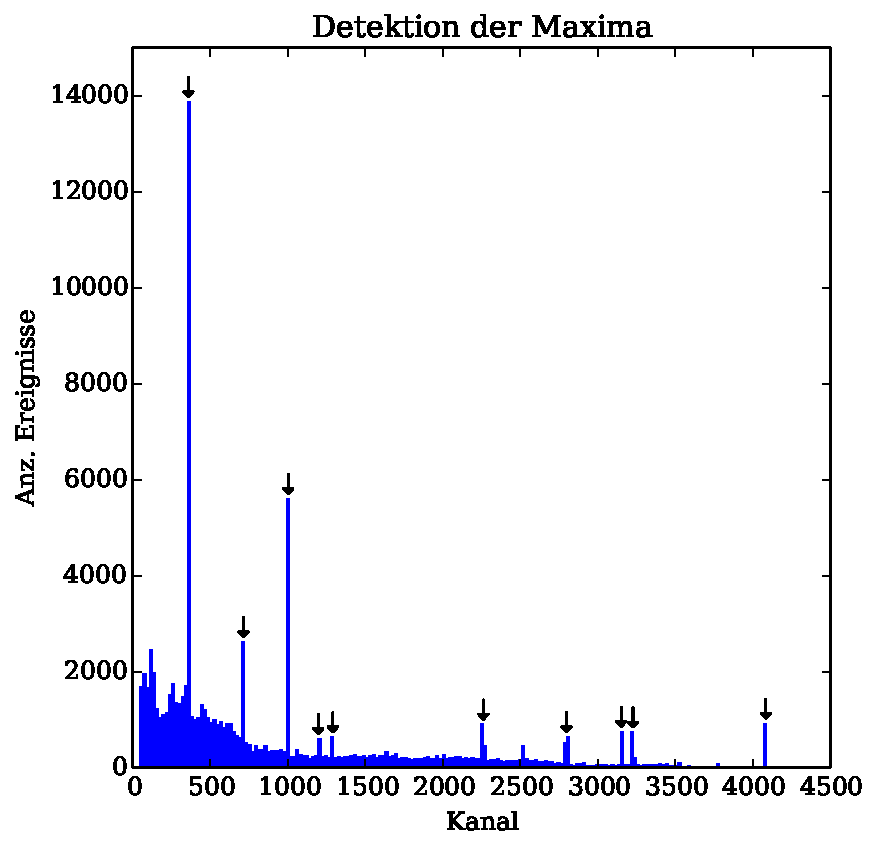
\includegraphics[width=1.0\linewidth]{img/02_maxima.pdf}
        \caption{
            Energiespektrum des $^{52}$Eu-Strahlers.
        }
        \label{fig:eu_uncalibrated}
    \end{subfigure}%
    \begin{subfigure}{.49\linewidth}
        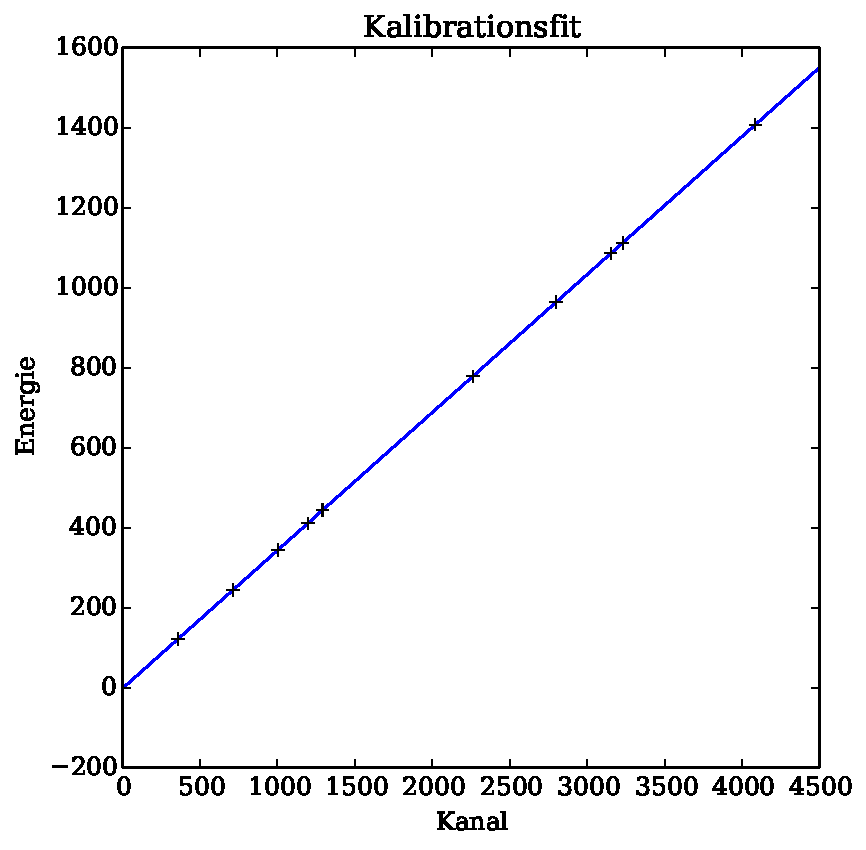
\includegraphics[width=1.0\linewidth]{img/03_calibration.pdf}
        \caption{
            Fit der Kalibrationsfunktion
        }
        \label{fig:calibration}
    \end{subfigure}
    \caption{
        Energiespektrum des $^{52}$Eu-Strahlers und Kalibrationsfunktion. Die Zur Kalibration genutzen Maxima sind in \ref{fig:eu_uncalibrated} durch einen Pfeil markiert.
    }
\end{figure}
Die unterschiedliche Messdauer wird mit einem Faktor $t_\text{leer} / t_\text{Eu}$ der Messdauer $t_\text{Eu}$ des $^{52}$Eu-Strahlers und $t_\text{leer}$ der Leermessung berücksichtigt.
Für die Kalibration werden die in Tabelle \ref{tab:maxima} aufgeführten Maxima gewählt und den jeweiligen Kanäle mit Hilfe von \eqref{eqn:kalibration} eine Energie zugeordnet. Der Fit der Kalibratinosfunktion ist in Abbildung \ref{fig:calibration} dargestellt.
Es ergeben sich die Koeffizienten
%
\begin{align*}
     m = \SI{345.22+-0.04}{keV/C} \qquad b = \SI{-1.82+-0.09}{keV} \,.
\end{align*}

Nach der Kalibration des Gerätes, kann die Effizienz $Q$ wie in Abschnitt \ref{sub:bestimmung_der_energie_und_der_aktivität_einer_gamma_quelle} beschrieben bestimmt werden. Mit Gleichungen \eqref{eqn:raumwinkel} ergibt sich ein Raumwinkelanteil des Detektors von
\begin{align*}
    \frac{\Omega}{4\pi} = \SI{1.575+-0.017}{\percent}\,.
\end{align*}
Die Gesamtaktivität $A_\text{ges}$ des Stahlers am Versuchstag berechnet sich mit Hilfe der bekannten Halbwertszeit $t_{1/2} = \SI{4943+-5}{d}$, der Anfangsaktivität $A_0 = \SI{4130+-60}{\becquerel}$ und der Zerfallszeit $\Delta t = \SI{5006}{d}$ zu
\begin{align*}
    A_\text{ges} = \SI{1500+-22}{\becquerel}\,.
\end{align*}
Für die Aktivität $A$, die im Detektor gemessen werden kann, gilt schließlich
\begin{align*}
    A &= \frac{\Omega}{4\pi}\cdot A_\text{ges}\,\\
    \Rightarrow \quad A &= \SI{23.6+-0.4}{\becquerel}\,.
\end{align*}
Unter Hinzunahme der bekannten Emissionswahrscheinlichkeiten kann nun wie in Gleichung \eqref{eqn:effizienz} beschrieben, eine Effizienzfunktion $Q(E)$ für den Detektor aufgestellt werden.
Eine Funktion $Q(E)$ der Form
\begin{align*}
    Q(E) = ae^{-bE}
\end{align*}
wird anschließend an die so erhaltenen Wertepaare $(Q,E)$ angepasst. Die oben aufgeführte Exponentialfunktion für $Q$ liefert im Gegensatz zu der im Skript vorgeschlagenen Potenzfunktion kleinere Fehler des Fits und wird daher bevorzugt. Der Fit ist in Abbildung \ref{fig:efficiency_fit} dargestellt und ergibt
\begin{align*}
    a &= \num{0.63+-0.26}\,, &\quad b &= \SI{1.8+-1.1}{\per eV} 2\,.
\end{align*}

\begin{figure}[htb]
    \centering
    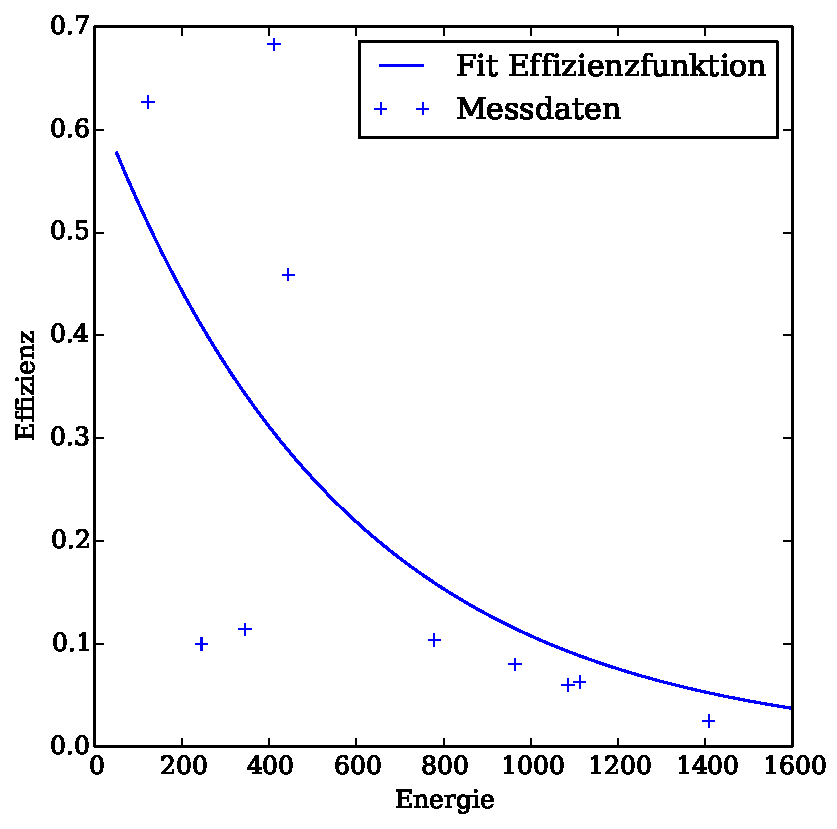
\includegraphics[width=0.5\linewidth]{img/05_efficiencies.pdf}
    \caption{
        Fit der Effizienzfunktion $Q$.
    }
    \label{fig:efficiency_fit}
\end{figure}

\begin{table}[htb]
    \centering
    \caption{
        Die für die Kalibration des Ge-Detektors verwendeten Maxima des $^{52}$Eu-Spektrums.
    }
    \label{tab:maxima}
    \begin{tabular}{%
        S[table-format=4.2]%
        S[table-format=2.1]%
        S[table-format=4.0]%
        S[table-format=5.0]%
        S[table-format=5.0]%
        S[table-format=2.1]%
    }
        \toprule
        {Energie [\si{keV}]} &
        {Emissionsw. [\si{\percent}]} &
        {Kanal} &
        {gemessen} &
        {erwartet} &
        {Effizienz [\si{keV}]} \\
        \midrule
        121.78 & 28.6 & 358  & 12544 & 20006 & 62.7 \\
        244.7  &  7.6 & 714  & 5319  & 53162 & 10.0 \\
        344.3  & 26.5 & 1003 & 2117  & 18537 & 11.4 \\
        411.12 & 02.2 & 1196 & 1051  &  1539 & 68.3 \\
        443.96 & 03.1 & 1291 & 996   &  2168 & 45.9 \\
        778.9  & 12.9 & 2262 & 938   &  9024 & 10.4 \\
        964.08 & 14.6 & 2798 & 817   & 10213 &  8.0 \\
        1085.9 & 10.2 & 3150 & 429   &  7135 &  6.0 \\
        1112.1 & 13.6 & 3227 & 598   &  9513 &  6.3 \\
        1408.0 & 21.0 & 4084 & 372   & 14690 &  2.5 \\
        \bottomrule
    \end{tabular}
\end{table}

\subsection{Bestimmung einiger Detektoreigenschaften} % (fold)
\label{sub:detektoreigenschaften}
Mit Hilfe eines $^{137}$Cs-Strahlers werden im folgenden Abschnitt einige Detektoreigenschaften bestimmt.
Das Spektrum des Stahlers ist in Abbildung \ref{fig:cs_spektrum} dargestellt.
\begin{figure}[htb]
    \centering
    \begin{subfigure}{0.49\linewidth}
        \centering
        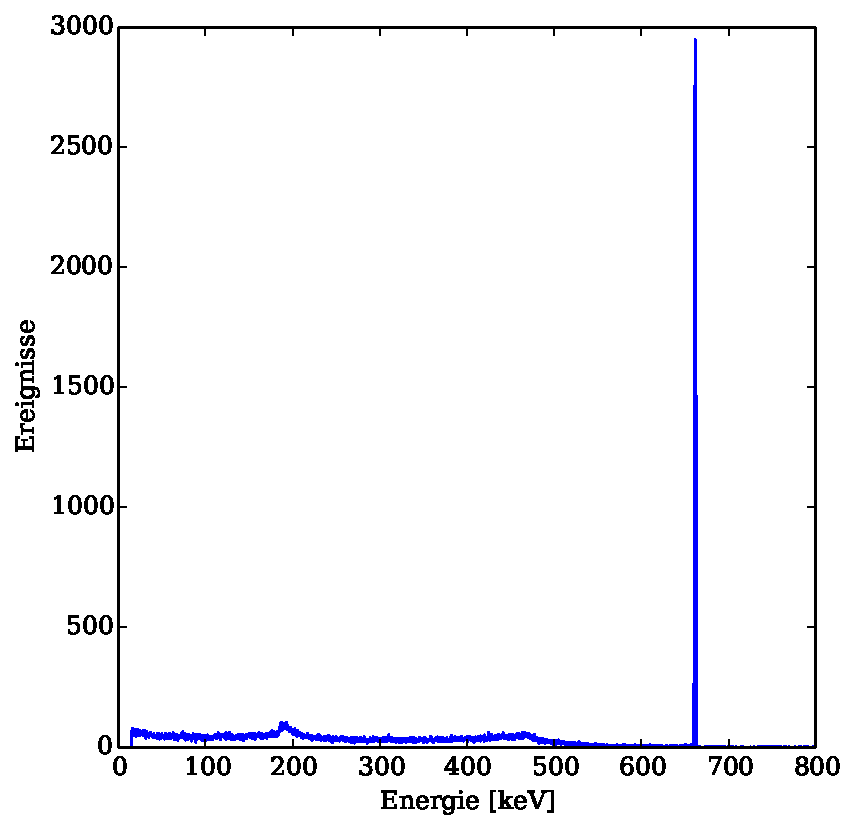
\includegraphics[width=1.0\linewidth]{img/06_caesium.pdf}
        \caption{
            Spektrum des $^{137}$Cs-Strahlers.
        }
        \label{fig:cs_spektrum}
    \end{subfigure}
    \begin{subfigure}{0.49\linewidth}
        \centering
        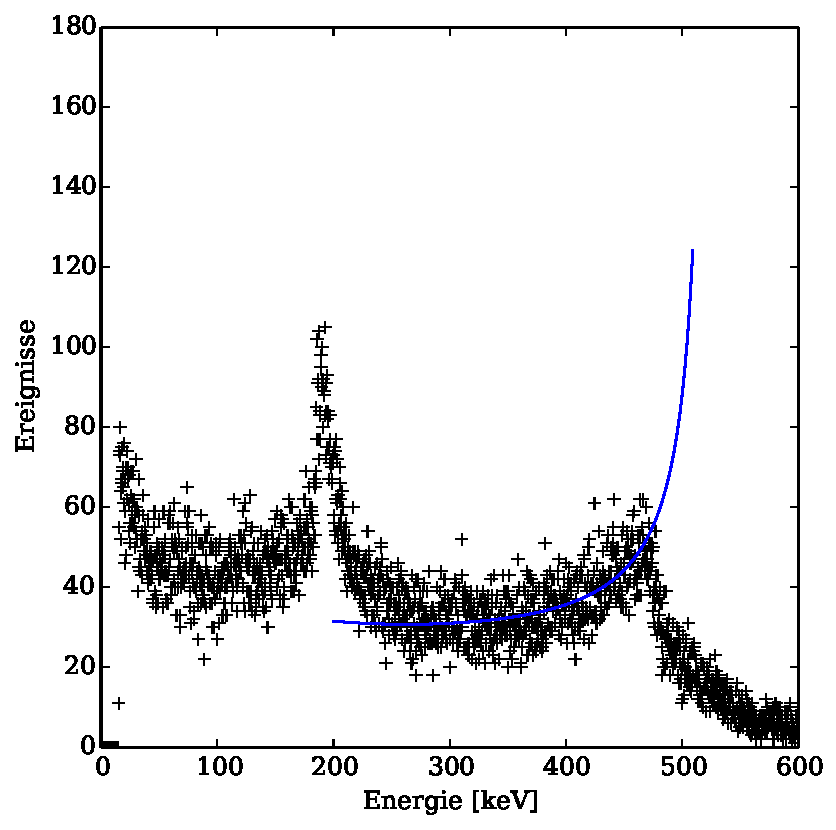
\includegraphics[width=1.0\linewidth]{img/06_caesium_zoomed.pdf}
        \caption{
            Compton-Streuung im $^{137}$Cs-Spektrum.
        }
        \label{fig:cs_spektrum_zoom}
    \end{subfigure}
    \caption{
        Spektrum des $^{137}$Cs-Strahlers. In Abbildung \ref{fig:cs_spektrum} ist das gesamte Spektrum inklusive deutlich erkennbarem Photo-Peak dargestellt.
        Abbildung \ref{fig:cs_spektrum_zoom} stellt den Bereich der Compton-Streuung dar, wobei jeder Datenpunkt aufgetragen ist und im rot markierten Bereich eine Funktion der Gestalt \eqref{eqn:compton} gefittet wird.
    }
\end{figure}

Zunächst wird der Photopeak des Spektrums genauer untersucht. Durch Fit einer Gaußfunktion im Bereich des Peaks lassen sich die genaue Lage und der Inhalt des Photopeaks bestimmen.
Für die Halb- und Zehntelwertsbreite $E_{1/2}$ und $E_{1/10}$ gilt mit Kenntnis der Breite $\sigma$ der Gaußverteilung
\begin{align*}
    E_{1/2} = 2\sigma\sqrt{\ln 2}\,,\quad E_{1/10} = 2\sigma\sqrt{\ln 10}\,.
\end{align*}
Der Fit ist in Abbildung \ref{fig:cs_gauss} dargestellt, er liefert folgende Werte für die Lage des Photopeaks $E_\gamma$, die Breiten $E_{1/2}$ und $E_{1/10}$, sowie die Anzahl $N$ der Ereignisse im Peak:
\begin{align*}
    E_\gamma &= \SI{661.623+-0.006}{keV} \,,&\quad N &= \num{12250+-110}\,,\\
    E_{1/2} &= \SI{2.752+-0.010}{keV}\,,&\quad E_{1/10} &= \SI{5.016+-0.018}{keV}\,,\\
    E_{1/2}^\text{t} &= \num{2.35} \sqrt{\num{0.1} E_\gamma E_\text{EL}} = \SI{1.03+-0.00}{keV}\,.
\end{align*}
Der Wert $E_{1/2}^\text{t}$ bezeichnet den im Skript erwähnten Theoriewert für die Halbwertsbreite.
Das Verhältnis der Halb- und Zehntelwertsbreiten beträgt
\begin{align*}
    \frac{E_{1/10}}{E_{1/2}} = \num{1.822+-0.010}\,,
\end{align*}
was mit dem erwarteten Verhältnis dieser Werte einer Gaußverteilung übereinstimmt.
\begin{figure}
    \centering
    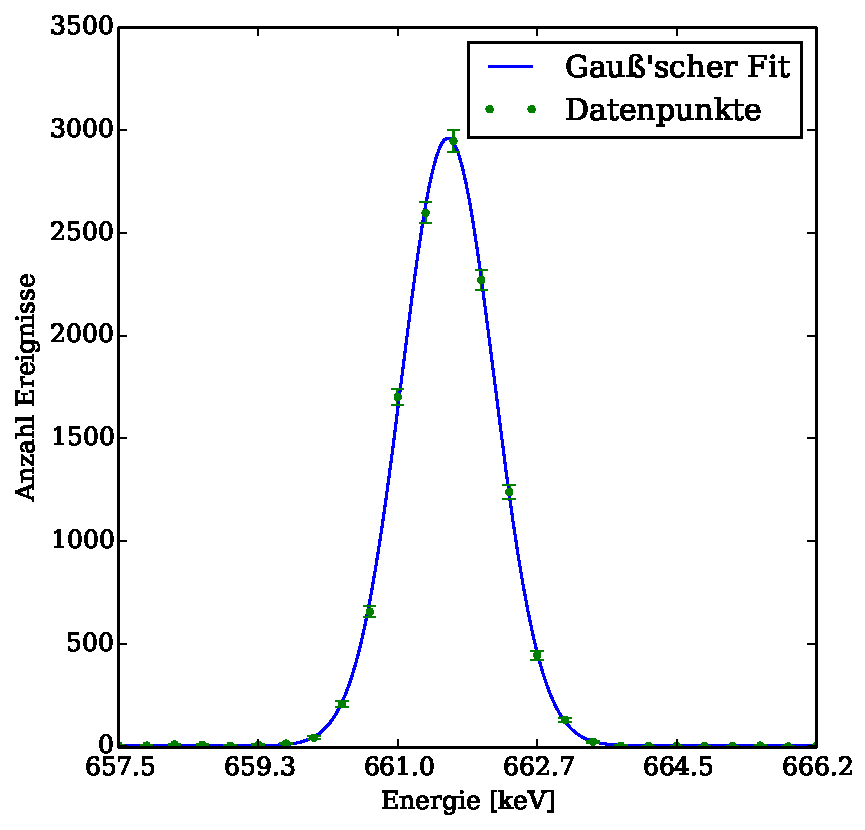
\includegraphics[width=0.5\linewidth]{img/06_caesium_fit.pdf}
    \caption{
        Spektrum des $^{137}$Cs-Strahlers im Bereich des Photo-Peaks. Durch die Datenpunkte wird eine Gaußfunktion gefittet, um die genaue Lage des Peaks zu bestimmen.
    }
    \label{fig:cs_gauss}
\end{figure}

Aschließend wird die Lage der Compton- und Rückstreukante bestimmt.
Auf Grund der Überlagerung der unterschiedlichen Wechselwirkungen im Detektor, ist die Bestimmung dieser Kanten durch einen Fit schwierig.
Stattdessen werden die Maxima der Energieverteilungen in den entsprechenden Bereichen mit der Position der Kanten identifiziert.
Dies liefert die Energie $E_\text{C}$ an der Compton-Kante, sowie $E_\text{R}$ an der Rückstreukante mit
\begin{align*}
    E_\text{C} &= \SI{463.537}{keV}\,, &\quad E_\text{R} &= \SI{192.887}{keV} \,,\\
    E_\text{C}^\text{t} &= \SI{477.302+-0.005}{keV}\,, &\quad E_\text{R}^\text{t} &= \SI{184.3206+-0.0005}{keV} \,.\\
\end{align*}
Die Theoretischen Werte $E^\text{t}$ lassen sich mit Hilfe der Formeln \eqref{eqn:compton_peak} und \eqref{eqn:rueckstreu_peak} berechnen. Für den Rückstreu-Peak wird ein Streuwinkel von $\phi = \SI{180}{\degree}$ angenommen.

Der Inhalt $I_\text{C}$ des Compton-Kontinuums wird durch numerische Integration der im Skript vorgeschlagenen Funktion für $\text{d}\sigma/\text{d}E$ von \SI{50}{keV} bis zum Compton-Peak bestimmt.
Die Paramter dieser Funktion werden dabei durch Fit an den in Abbildung \ref{fig:cs_spektrum_zoom} markierten Bereich bestimmt. Damit ergibt sich
\begin{align*}
    I_\text{C} = \num{47190+-220}\,.
\end{align*}

Abschließend wird das Verhältnis der Anzahl an Ereignissen im Photo-Peak und dem Compton-Kontinuum untersucht.
Mit Hilfe der Extinktionskoeffizienten $\mu$ für Compton- und Photo-Effekt lassen sich unter Kenntnis der Detektorabmessungen $D$ die Absorptionswahrscheinlichkeiten $W(D)=1-\exp(-\mu D)$ für beide Effekte vorhersagen. Die Koeffizienten $\mu$ werden in Abbildung \ref{german} abgelesen:
\begin{align*}
    \mu_\text{C} &= \num{0.42}\,, &\quad \mu_\text{P} &= \num{0.008}\,,\\
    \Rightarrow \quad W_\text{C} &\approx \SI{80}{\percent} &\quad W_\text{P} &\approx \SI{3}{\percent} \,.
\end{align*}
Das Compton-Kontinuum sollte somit im Vergleich zum Photo-Peak die etwa \num{27}-fache Anzahl an Ereignissen beinhalten.
Die gemessenen Inhalte ergeben jedoch ein Verhältnis von etwa $4:1$.
% subsection bestimmung_einiger_detektoreigenschaften (end)

\subsection{Aktivität einer $^{133}$Ba-Quelle} % (fold)
\label{sub:ba_quelle}
In diesem Abschnitt wird das Spektrum einer $^{133}$Ba-Quelle vermessen. Anschließend wird der Inhalt der einzelnen Peaks im Spektrum bestimmt, woraus unter Berücksichtigung der Effizienzfunktion $Q$ und dem Raumwinkelanteil $\Omega$ des Detektors auf die Aktivität $A_\text{ges}$ der Quelle geschlossen werden kann.
Das aufgenommene Spektrum ist in Abbildung \ref{fig:ba_spektrum} gezeigt.
Es werden die in Tabelle \ref{tab:barium} aufgeführten Peaks des Spektrums mit den bekannten Gamma-Linien aus dem Skript identifiziert.
Mit Hilfe von Gleichung \eqref{eqn:effizienz} kann dann die Aktivität $A$ der Quelle als Parameter eine linearen Ausgleichsrechnung bestimmt werden.
Der Fit für die Bestimmung von $A_\text{ges}$ ist in Abbildung \ref{fig:barium_aktivitaet} dargestellt und liefert
\begin{align*}
    A_\text{ges} = \SI{970+-190}{\becquerel}\,.
\end{align*}
\begin{figure}
    \centering
    \begin{subfigure}{0.49\linewidth}
        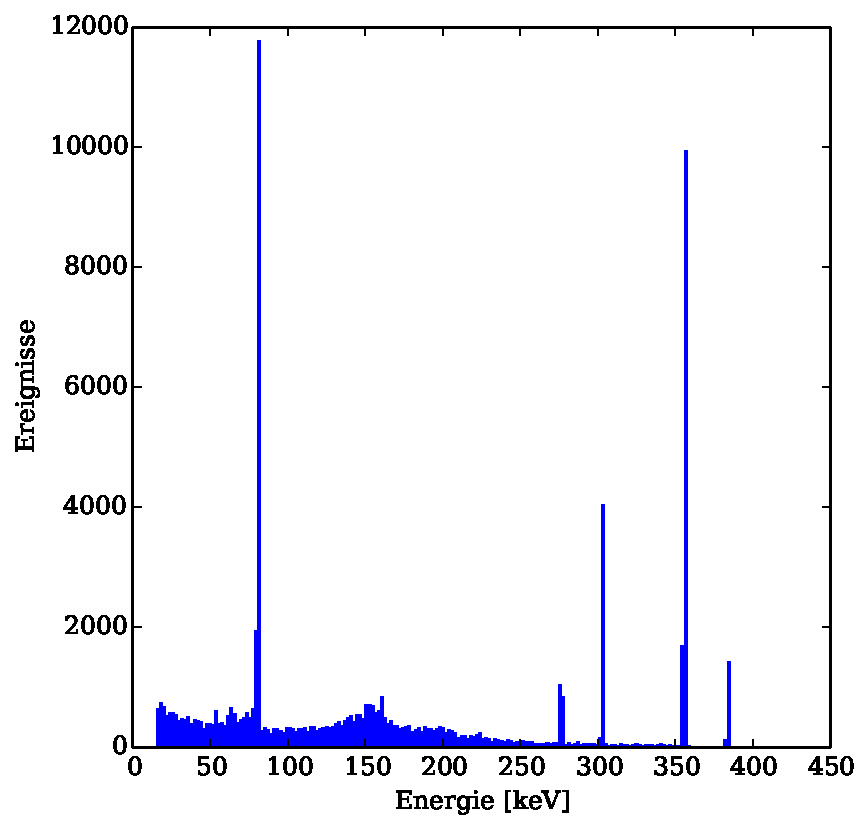
\includegraphics[width=0.5\linewidth]{img/07_barium.pdf}
        \caption{
            Spektrum des vermessenen $^{133}$Ba-Strahlers.
        }
        \label{fig:ba_spektrum}
    \end{subfigure}
    \begin{subfigure}{0.49\linewidth}
        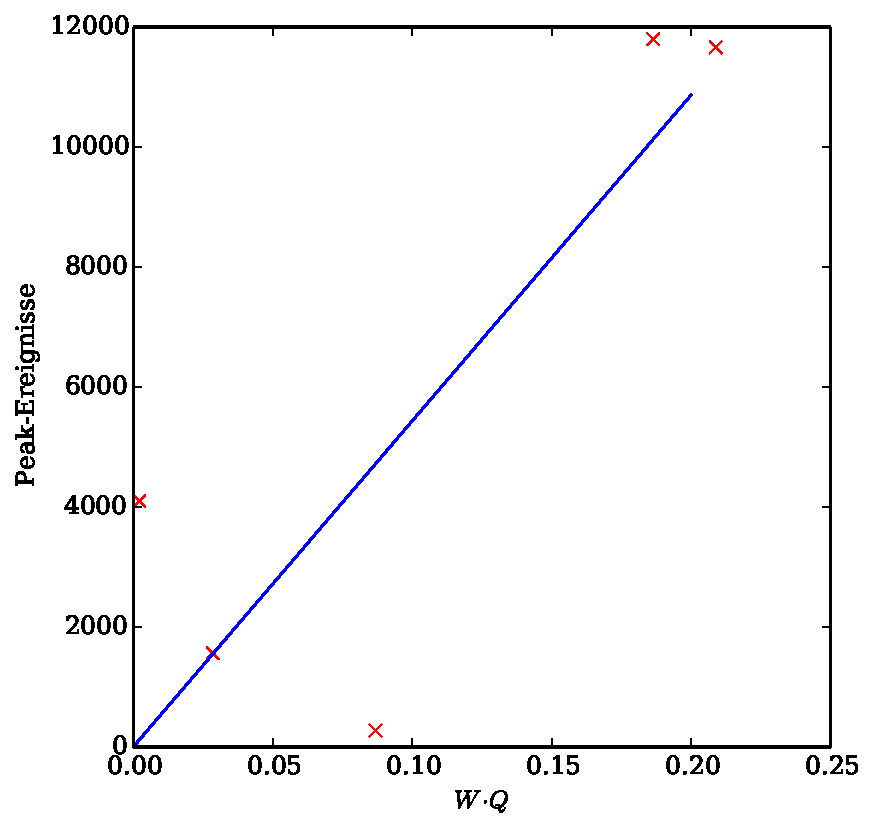
\includegraphics[width=0.5\linewidth]{img/07_barium_activity.pdf}
        \caption{
            Fit zur Bestimmung der Aktivit der $^{133}$Ba-Quelle.
        }
        \label{fig:barium_aktivitaet}
    \end{subfigure}
\end{figure}
\begin{table}
    \centering
    \label{tab:barium}
    \caption{Barium}
    \begin{tabular}{%
        S[table-format=3.1]%
    }
        \toprule
        {Peak [\si{keV}]} \\
        \midrule
        \bottomrule
    \end{tabular}
\end{table}

\subsection{Radioaktivität von Holzkohlebrikkets} % (fold)
\label{sub:holzkohle}

% subsection holzkohle (end)

% subsection ba_quelle (end)
